%% -*- coding:utf-8 -*-
\documentclass[10pt,pdf,hyperref={unicode}]{beamer}
\input ./preamble.tex
\usetheme{Warsaw}
\title[Quantum cryptography]{Classical
  cryptography\\Quantum cryptography}
\author{Ivan Murashko}
%\institute{Санкт Петербургский Государственный Политехнический Университет}
\date{}
\begin{document}

\begin{frame}
\titlepage
\end{frame}


\section{Introduction}

\begin{frame}{Introduction}
\begin{itemize}
\item Classic cryptography
  \begin{itemize}
    \item Caesar cipher
    \item Vernam cipher (one-time pad)
    \item Key distribution (Diffie-Hellman)
  \end{itemize}
\item Quantum cryptography
  \begin{itemize}
    \item Einstein–Podolsky–Rosen paradox
  \end{itemize}
\end{itemize}
\end{frame}

\section{Classic cryptography}

\begin{frame}{Lorenz cipher, WWII}
 \begin{figure} 
   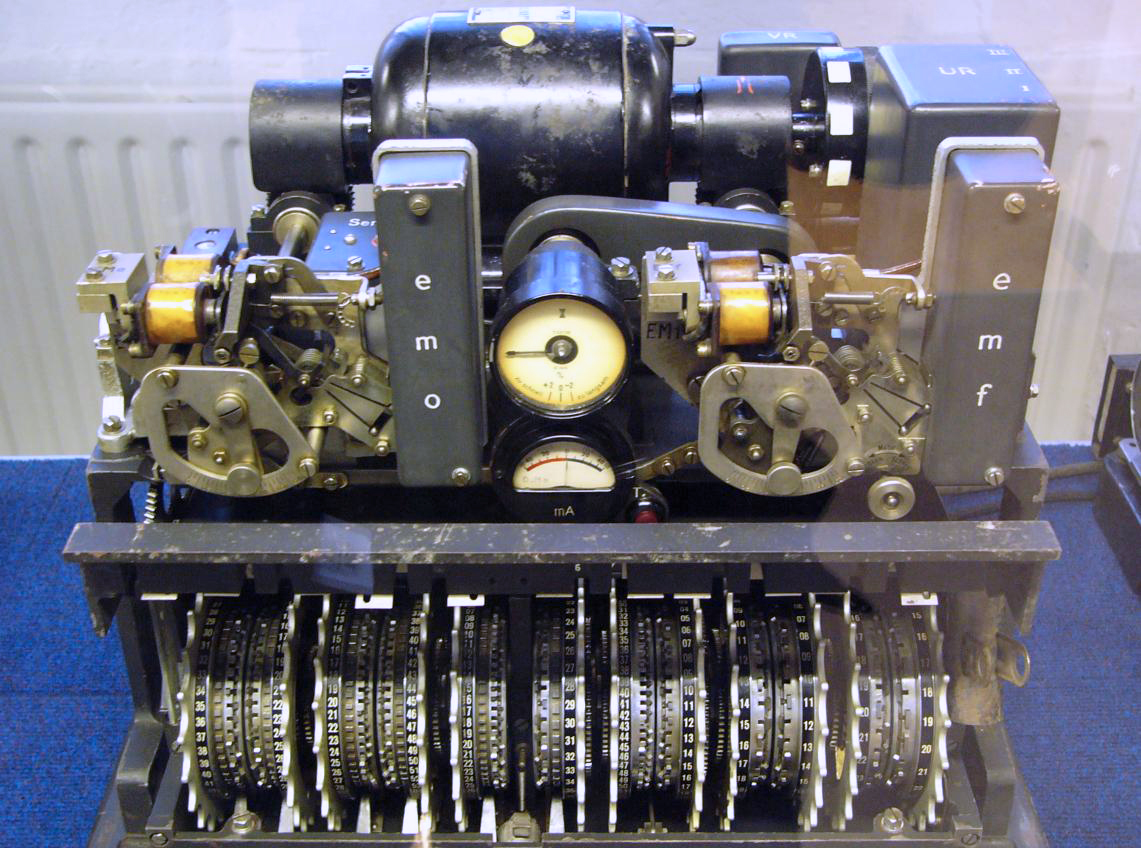
\includegraphics[width=90mm,scale=0.5]{class_crypto.jpg}
  \end{figure}
\end{frame}


\begin{frame}{Caesar cipher}
 \begin{figure} 
   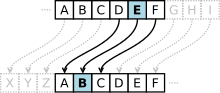
\includegraphics[width=90mm,scale=0.5]{caesar_cipher.png}
  \end{figure}
\end{frame}

\begin{frame}{Hack the caesar cipher}
 \begin{figure} 
   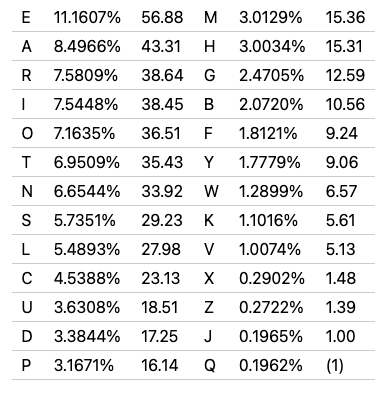
\includegraphics[width=90mm,scale=0.5]{english_letters}
  \end{figure}
\end{frame}

\begin{frame}{Perfect security}
 \begin{figure} 
   Is there a cipher that is unbreakable?
 \end{figure}
\end{frame}

\begin{frame}{Shannon 1949}
 \begin{figure} 
   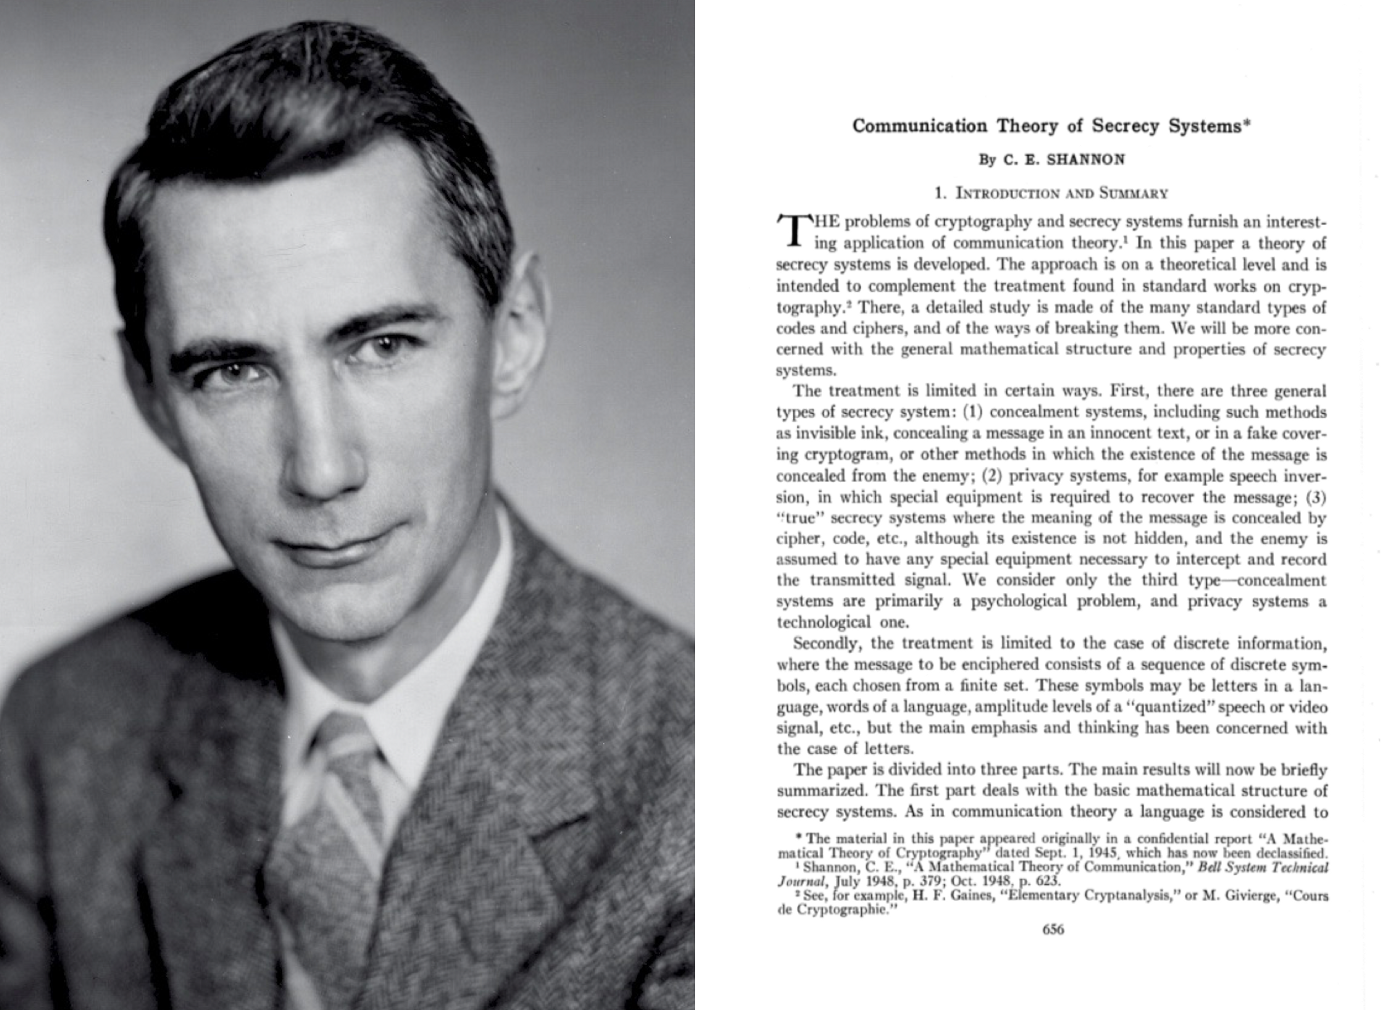
\includegraphics[width=90mm,scale=0.5]{shannon.png}
 \end{figure}
\end{frame}

\begin{frame}{Vernam cipher, one-time pad, 1917}
  \begin{table}
    \centering
    \begin{tabular}{|c|c|c|}
      \hline
      $t$ & $k$ & $c = t \oplus k$ \\ \hline
      0  & 0 & 0 \\
      0  & 1 & 1 \\
      1  & 0 & 1 \\
      1  & 1 & 0 \\ \hline
    \end{tabular}
    \caption{XOR $t \oplus k$}
    \label{tblXOR}
  \end{table}
  Thus you you have a text ($t$) and key ($k$) then you can get an
  encoded text as follows
  \[
  c = t \oplus k
  \]
  original text can be restored as
  \[
  t = c \oplus k
  \]  
\end{frame}

\begin{frame}{Key distribution. Discrete log}
  \[
  x = ind_g\left(a\right) \mod{p}
  \]
  min $x$ such that
  \[
  g^x \equiv a \mod{p}
  \]
\end{frame}

\begin{frame}{Key distribution. Diffie-Hellman}
  Known data: $g$, $p$
  
  Alice choose random $a$ and calculates
  \[
  A \equiv g^a \mod{p}
  \]

  Bob choose random $b$ and calculates
  \[
  B \equiv g^b \mod{p}
  \]

  Alice and Bob exchange the $A$ and $B$ and calculate $K$ as
  \[
  K \equiv B^a \mod{p}
  \]
  or
  \[
  K \equiv A^b \mod{p}
  \]  
\end{frame}


\section{Quantum cryptography}

\begin{frame}{Base principles}
  \begin{enumerate}
  \item Measurement is random
  \item Alice and Bob measurements are correlated
  \item No-cloning theorem
  \end{enumerate}
\end{frame}



\begin{frame}{Heisenberg inequality}
  \[
  \Delta p \Delta q \ge \frac{\hbar}{2}
  \]
\end{frame}


\begin{frame}{Einstein–Podolsky–Rosen paradox}
 \begin{figure} 
   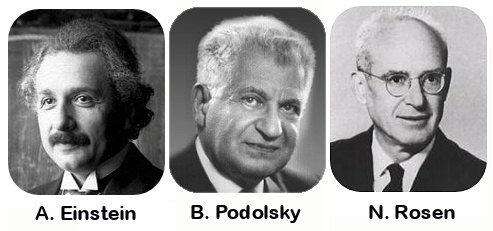
\includegraphics[width=90mm,scale=0.5]{epr.jpg}
  \end{figure}
\end{frame}

\begin{frame}{Bell experiment. Classical case}
\[
f = \frac{1}{2}\left(
a b + a' b + a b' - a' b'
\right), a,a',b,b' \in \{-1, +1\}.
\]
therefore
\(
f \in \{-1, +1\}
\)
and
\(
\left|\left<f\right>\right| \le 1
\)
\end{frame}

\begin{frame}{Bell experiment. Quantum case}
\[
\left|\left<f\right>\right| = \sqrt{2} > 1
\]
\end{frame}



\begin{frame}{Questions}
 \begin{figure} 
   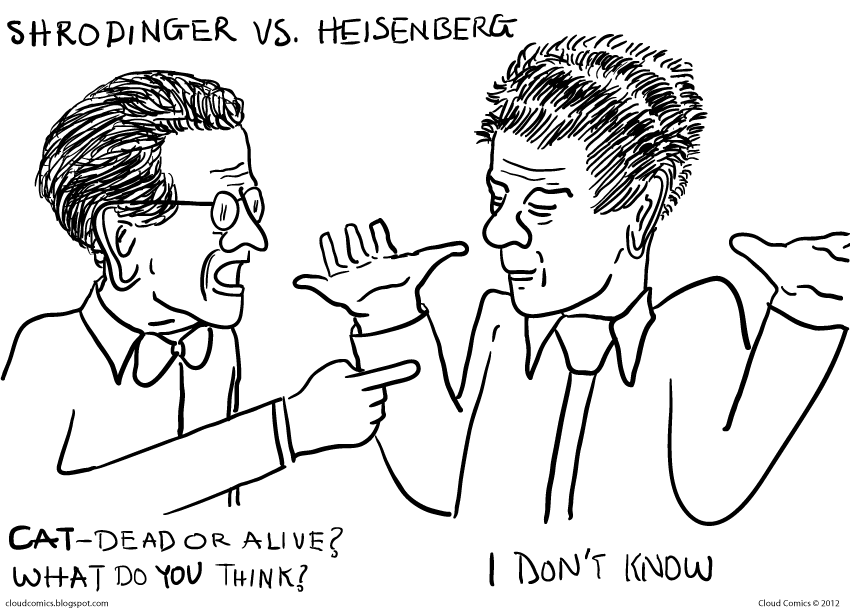
\includegraphics[width=90mm,scale=0.5]{questions.png}
  \end{figure}
\end{frame}

\end{document}
